\documentclass[10pt]{article}
\usepackage[margin=0.8in]{geometry}
\usepackage[utf8]{inputenc}
\usepackage[T1]{fontenc}
\usepackage{graphicx}
\usepackage[export]{adjustbox}
\usepackage{amsmath}
\usepackage{amsfonts}
\usepackage{amssymb}
\usepackage[version=4]{mhchem}
\usepackage{stmaryrd}
\usepackage{bbold}
\usepackage{fixltx2e}
\usepackage{caption}
\usepackage{mathtools}
\usepackage[parfill]{parskip}
\usepackage{float}
\usepackage{amsmath}

\usepackage[framemethod=TikZ]{mdframed}
\colorlet{shadecolor}{orange!15}
\usepackage{xcolor}
\usepackage{amsthm}
\usepackage{framed}



\begin{document}



\title{Lecture 16-17: Numerical Inverse Kinematics Algorithms}
\date{Oct. 17, 2023 \quad  \quad Oct. 19, 2023}
\author{Wanxin Jin}
\maketitle

Recall the problem of Inverse Kinematics (IK): given $\boldsymbol{x}_{d}$ (the desired end-effector pose in the operational space), we want to find the joint value $\boldsymbol{q}$ such that $\boldsymbol{k}(\boldsymbol{q})=\boldsymbol{x}_d$. Here, $\boldsymbol{k}(\cdot)$ is the forward kinematics.

To solve the above IK, we define the following operational space error between the desired $\boldsymbol{x}_{d}$  and the current end-effector pose $\boldsymbol{x}_{e}$: 



$$
\boldsymbol{e}=\boldsymbol{x}_{d}-\boldsymbol{x}_{e}
$$

Consider the time derivative

$$
\dot{\boldsymbol{e}}=\dot{\boldsymbol{x}}_{d}-\dot{\boldsymbol{x}}_{e}=\dot{\boldsymbol{x}}_{d}-\boldsymbol{J}_{A}(\boldsymbol{q}) \dot{\boldsymbol{q}}
$$

The above is called \emph{error dynamics} (an Ordinary Differential Equation), as it shows the profile of the operational space error $\boldsymbol{e}(t)$ over time $t$. Here, $\dot{\boldsymbol{q}}$ can be viewed as the control input.
From a control perspective, we want to find a feedback control law 

$$
\dot{\boldsymbol{q}}= \text{Controller}({\boldsymbol{x}}_d, \dot{\boldsymbol{x}}_d,  {\boldsymbol{q}}, {\boldsymbol{e}})
$$

such that, when plug the controller to the error dynamics,  $\boldsymbol{e}(t)\rightarrow 0$ as $t\rightarrow \infty$. The different controllers leads to different numerical IK algorithms.



\section{Controller 1: Jacobian (Pseudo-)Inverse or Newton-Raphson Method}



Let's define  $
\dot{\boldsymbol{q}}= \text{Controller}({\boldsymbol{x}}_d, \dot{\boldsymbol{x}}_d,  {\boldsymbol{q}}, {\boldsymbol{e}})
$ specifically as 

$$
\dot{\boldsymbol{q}}=
\begin{cases}
\boldsymbol{J}_{A}^{-1}(\boldsymbol{q})\left(\dot{\boldsymbol{x}}_{d}+\boldsymbol{K} \boldsymbol{e}\right)  \quad\quad\text{for non-redundant manipulators} \\
\boldsymbol{J}_{A}^{\dagger}\left(\dot{\boldsymbol{x}}_{d}+\boldsymbol{K e}\right)+\left(\boldsymbol{I}_{n}-\boldsymbol{J}_{A}^{\dagger} \boldsymbol{J}_{A}\right) \dot{\boldsymbol{q}}_{0} \quad\quad\text{for redundant manipulators}
\end{cases}
$$



Submitting the above controllers into the error dynamics, it easy to verify that


$$
\dot{\boldsymbol{e}}+\boldsymbol{K} \boldsymbol{e}=0 .
$$

If $\boldsymbol{K}$ is a positive definite (usually diagonal) matrix, the above is asymptotically stable. The error tends to zero along the trajectory with a convergence rate that depends on the eigenvalues of  $\boldsymbol{K}$.


\begin{shaded}

\textbf{Background from Linear Control Systems course}


Generally, given an ordinary differential equation (ODE)  $$
\dot{\boldsymbol{e}}+\boldsymbol{K} \boldsymbol{e}=0 .
$$ the solution $\boldsymbol{e}(t)$ to the ODE is 

$$
\boldsymbol{e}(t)=e^{\boldsymbol{-K}t}\boldsymbol{e}(0)
$$

In particular, if $\boldsymbol{K}$ is diagonal, say $$
\boldsymbol{K}=\begin{bmatrix}
\lambda_1& & &\\
&\lambda_2 & & \\
& & \ddots &\\
& & & \lambda_r
\end{bmatrix},
$$
Then, the solution is 
\begin{equation}
    \boldsymbol{e}(t)=\begin{bmatrix}
e^{-\lambda_1t}& & &\\
&e^{-\lambda_2t} & & \\
& & \ddots &\\
& & & e^{-\lambda_rt}
\end{bmatrix}\boldsymbol{e}(0)
\end{equation}
Therefore, only if $\lambda_1, \lambda_2, ...\lambda_r>0$, $\boldsymbol{e}(t)\rightarrow \boldsymbol{0}$ as $t\rightarrow \infty$. 

\end{shaded}










The block scheme corresponding to the IK algorithm is illustrated below, where $\boldsymbol{k}(\cdot)$ indicates the direct kinematics function. 


\begin{figure}[H]
    \centering
    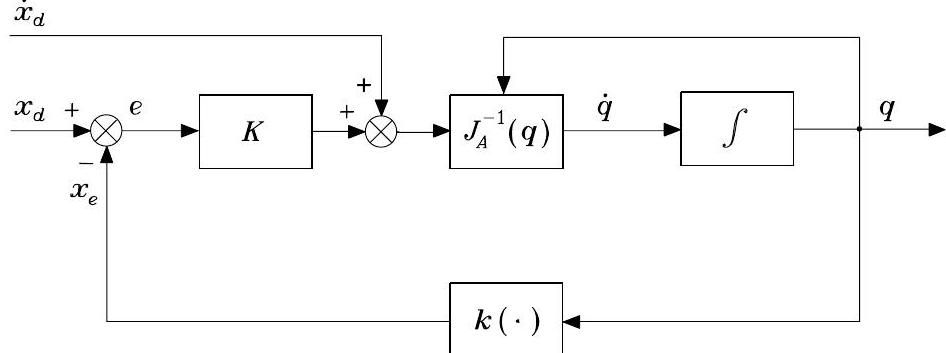
\includegraphics[max width=0.5\textwidth]{diff_kinematics/IK_jacobian_inverse}
    \caption{IK algorithm with Jacobian inverse}
    \label{l2-2.fig1}
\end{figure}

\begin{shaded}
\textbf{Another perspective to look at the above Jacobian Inverse Controller is through Newton-Raphson method in solving nonlinear equations}

Specifically, consider the following nonlinear equation from kinematics

$$
\boldsymbol{k}(\boldsymbol{q})=\boldsymbol{x}_d
$$

given the desired end-effector pose $\boldsymbol{x}_d$. 

Assume we are given the current initial guess $\boldsymbol{q}_t$. One can approximate the above kinematics at $\boldsymbol{q}_k$ using the first-order Tyler expression:

$$
\boldsymbol{k}(\boldsymbol{q})\approx\boldsymbol{t}(\boldsymbol{q}_t)+\boldsymbol{J}_{A}(\boldsymbol{q}_t)(\boldsymbol{q}-\boldsymbol{q}_t)=\boldsymbol{x}_d
$$

By solving the above equation for $\boldsymbol{q}$, one can obtain the next updated guess 

$$
\boldsymbol{q}_{t+1}=\boldsymbol{q}_t+\text{inv}\left(\boldsymbol{J}_{A}(\boldsymbol{q}_t)\right)(\boldsymbol{x}_d-\boldsymbol{t}(\boldsymbol{q}_t))=\boldsymbol{q}_t+\text{inv}\left(\boldsymbol{J}_{A}(\boldsymbol{q}_t)\right)\boldsymbol{e}_t
$$

where $\text{inv}$ is the general inverse operation (inverse for square matrix or pseudo-inverse for non-square matrix). Typically, one also needs a step size before $\text{inv}\left(\boldsymbol{J}(\boldsymbol{q}_t)\right)$ to stabilize the Newton-Raphson algorithm.  The above results can be considered as the discrete-time interpretation of the Jacobian Inverse IK algorithm if $\dot{\boldsymbol{x}}_d=\boldsymbol{0}$.
\end{shaded}



\section{Controller 2: Jacobian Transpose or Gradient-Based Method}

\begin{shaded}
    \textbf{Background from Linear Control Systems course: Lyapunov Stability}

Consider the following error dynamics (ODE)
$$
\dot{\boldsymbol{e}}(t)=\boldsymbol{f}(\boldsymbol{e}(t)),\quad \text{given}\quad \boldsymbol{x}(0)
$$

If there exists  a Lyapunov function $V(\boldsymbol{e})$ such that 
\begin{itemize}
    \item $ 
V(\boldsymbol{e})>0 \quad \forall \boldsymbol{e} \neq \mathbf{0}
$
\item $
V(\mathbf{0})=0 \quad \text{only for} \quad \boldsymbol{e}=\boldsymbol{0}
$
\item $
\dot{V}=\frac{dV}{dt}=(\frac{d V}{d\boldsymbol{e}})^T\dot{\boldsymbol{e}}=(\frac{d V}{d\boldsymbol{e}})^T \boldsymbol{f}(\boldsymbol{e}(t))<0 \quad \forall \boldsymbol{e} 
$
\end{itemize}
then, ${\boldsymbol{e}}(t)\rightarrow \boldsymbol{0}$ as $t\rightarrow \infty$ (the error is converging).

\end{shaded}

Consider $\dot{\boldsymbol{x}}_{d}=\mathbf{0}$.
Let's use Lyapunov function to find another controller such that the error dynamics is converging. Let's choose  Lyapunov function as

$$
V(\boldsymbol{e})=\frac{1}{2} \boldsymbol{e}^{T} \boldsymbol{K} \boldsymbol{e}
$$

where $\boldsymbol{K}$ is a symmetric positive definite matrix. Obviously,

$$
V(\boldsymbol{e})>0 \quad \forall \boldsymbol{e} \neq \mathbf{0}, \quad V(\mathbf{0})=0 \quad \text{only for} \quad \boldsymbol{e}=\boldsymbol{0}
$$

Differentiating $V(\boldsymbol{e})$ with respect to time gives

$$
\dot{V}=\boldsymbol{e}^{T} \boldsymbol{K} \dot{\boldsymbol{x}}_{d}-\boldsymbol{e}^{T} \boldsymbol{K} \dot{\boldsymbol{x}}_{e}=\boldsymbol{e}^{T} \boldsymbol{K} \dot{\boldsymbol{x}}_{d}-\boldsymbol{e}^{T} \boldsymbol{K} \boldsymbol{J}_{A}(\boldsymbol{q}) \dot{\boldsymbol{q}}
$$


At this point, since $\boldsymbol{\dot{x}}_d=\boldsymbol{0}$, if we choose

$$
\dot{\boldsymbol{q}}=\boldsymbol{J}_{A}^{T}(\boldsymbol{q}) \boldsymbol{K} \boldsymbol{e}
$$

This leads to

$$
\dot{V}=-\boldsymbol{e}^{T} \boldsymbol{K} \boldsymbol{J}_{A}(\boldsymbol{q}) \boldsymbol{J}_{A}^{T}(\boldsymbol{q}) \boldsymbol{K} \boldsymbol{e}
$$

 $\dot{V}$ is negative definite, under the assumption of full rank for $\boldsymbol{J}_{A}(\boldsymbol{q})$. $\dot{V}<0$ with $V>0$ implies the error dynamics will converge/stabilize to  $\boldsymbol{e}=\mathbf{0}$, according to Lyapunov Stablity.  The block scheme is illustrated below.

\begin{figure}[H]
    \centering
    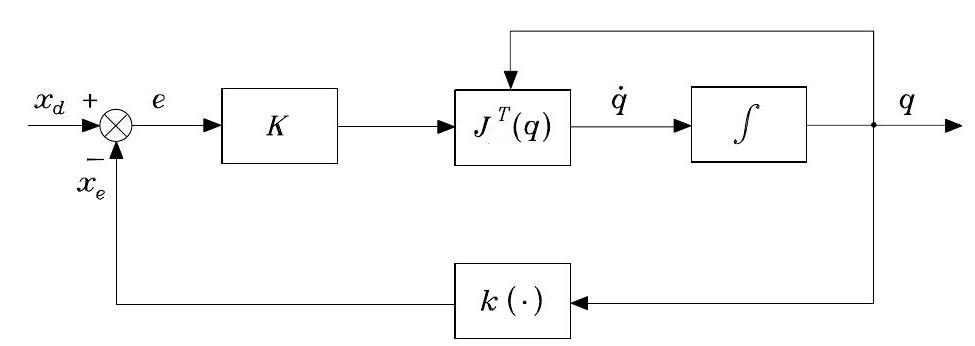
\includegraphics[max width=0.5\textwidth]{diff_kinematics/IK_jacobian_transpose.jpg}
    \caption{Block scheme of the inverse kinematics algorithm with Jacobian transpose}
    \label{l2-2.fig2}
\end{figure}


\begin{shaded}

\textbf{Another perspective to look at  Jacobian transpose controller via gradient-based optimization}

Specifically, when $\dot{\boldsymbol{x}}_d=\boldsymbol{0}$, consider we want to find the joint value $\boldsymbol{q}$ by minimizing the error of 

$$
\min_{\boldsymbol{q}}\quad\frac{1}{2}||\boldsymbol{k}(\boldsymbol{q})-\boldsymbol{x}_d||^2
$$

The gradient descent to update current guess $\boldsymbol{q}_k$ to next $\boldsymbol{q}_{k+1}$

$$
\boldsymbol{q}_{k+1}=\boldsymbol{q}_{k}-\alpha{\left(\frac{d\boldsymbol{k}(\boldsymbol{q})}{d\boldsymbol{q}}\bigg\rvert_{\boldsymbol{q}=\boldsymbol{q}_k}\right)}^{T}(\boldsymbol{k}_{A}(\boldsymbol{q})-\boldsymbol{x}_d)=\boldsymbol{q}_{k}+\alpha{\boldsymbol{J}(\boldsymbol{q}_k)}^{T}\boldsymbol{e}_k
$$

where $\alpha$ is the gradient step size. The above
results can be considered as the discrete-time interpretation of the Jacobian transpose IK algorithm if  $\boldsymbol{\dot{x}}_d=0$.


\end{shaded}


\subsection*{More Discussion (Optional)}

 When  $\dot{\boldsymbol{x}}_{d} = \mathbf{0}$ and  $\mathcal{N}\left(\boldsymbol{J}_{A}^{T}\right) \neq \emptyset$, $\dot{V}$ is only negative semi-definite, since $\dot{V}=0$ for $\boldsymbol{e} \neq \mathbf{0}$ with $\boldsymbol{K} \boldsymbol{e} \in \mathcal{N}\left(\boldsymbol{J}_{A}^{T}\right)$. In this case, the algorithm can get stuck at $\dot{\boldsymbol{q}}=\mathbf{0}$ with $\boldsymbol{e} \neq \mathbf{0}$.



When  $\dot{\boldsymbol{x}}_{d} \neq \mathbf{0}$, in order to obtain $\dot{V}<0$ also in this case, it would be sufficient to choose 

$$
\dot{\boldsymbol{q}}=
\begin{cases}
\boldsymbol{J}_{A}^{-1}\left(\dot{\boldsymbol{x}}_{d}+\boldsymbol{K} \boldsymbol{e}\right)  \quad\quad\text{for non-redundant manipulators} \\
\boldsymbol{J}_{A}^{\dagger}\left(\dot{\boldsymbol{x}}_{d}+\boldsymbol{K e}\right)+\left(\boldsymbol{I}_{n}-\boldsymbol{J}_{A}^{\dagger} \boldsymbol{J}_{A}\right) \dot{\boldsymbol{q}}_{0} \quad\quad\text{for redundant manipulators}
\end{cases}
$$

which is exactly the Jacobian inverse controller introduced in the first section. 

Furthermore, we have the following comments on the above Jacobian transpose controller.

\begin{itemize}
    \item  In the case of kinematic singularities, we have to use Jacobian transpose IK because it does not require the inverse/pseudo-inverse of the Jacobian

\item  Although the Jacobian transpose IK cannot guarantee the convergence of the error dynamics when $\dot{\boldsymbol{x}}_{d} \neq \mathbf{0}$, the tracking error $\boldsymbol{e}(t)$ is norm-bounded. This is because, when the error norm is small, the linear term (the first term in $\dot{V}(t)$) prevails in the second quadratic term; when otherwise, the quadratic term dominates, dragging the error to the small norm.

\end{itemize}



\section{Definition of Orientation Error}

Both IK algorithms above require the definition of the error in the operational space (note that we have used the analytical Jacobian instead of the geometric Jacobian). This is natural for the position part of the end-effector

$$
\boldsymbol{e}_{P}=\boldsymbol{p}_{d}-\boldsymbol{p}_{e}(\boldsymbol{q})
$$

where $\boldsymbol{p}_{d}$ and $\boldsymbol{p}_{e}$ denote respectively the desired and computed end-effector positions. Its time derivative is

$$
\dot{\boldsymbol{e}}_{P}=\dot{\boldsymbol{p}}_{d}-\dot{\boldsymbol{p}}_{e} .
$$



However, the problem arises when we consider defining the orientation error, which depends on the representation of the orientation. In the following, let's consider the typical types of orientation representation and its error.







\subsection{Euler-Angles Error}
The orientation error using Euler angles is 

$$
\boldsymbol{e}_{O}=\boldsymbol{\phi}_{d}-\boldsymbol{\phi}_{e}(\boldsymbol{q})
$$

where $\boldsymbol{\phi}_{d}$ and $\boldsymbol{\phi}_{e}$ denote respectively the desired and computed set of Euler angles. Its time derivative is

$$
\dot{\boldsymbol{e}}_{O}=\dot{\boldsymbol{\phi}}_{d}-\dot{\boldsymbol{\phi}}_{e}
$$

The analytical Jacobian for ZYZ-Euler angles was given in previous lectures: $\boldsymbol{J}_{A}=\boldsymbol{T}^{-1}\boldsymbol{J}$ with $\boldsymbol{J}$ being the geometric jacobian and 

$$
\boldsymbol{T}\left(\phi_{e}\right) =\left[\begin{array}{ccc}
0 & -s_{\varphi} & c_{\varphi} s_{\vartheta} \\
0 & c_{\varphi} & s_{\varphi} s_{\vartheta} \\
1 & 0 & c_{\vartheta}
\end{array}\right] .
$$




\subsection{Angle-Axis Error (Optional)}

If the desired orientation  of the end-effector is given in rotation matrix $\boldsymbol{R}_{d}=\left[\begin{array}{lll}\boldsymbol{n}_{d} & \boldsymbol{s}_{d} & \boldsymbol{a}_{d}\end{array}\right]$ and current end-effector's rotation matrix is $\boldsymbol{R}_{e}(\boldsymbol{q})=\left[\begin{array}{lll}\boldsymbol{n}_{e}(\boldsymbol{q}) & \boldsymbol{s}_{e}(\boldsymbol{q}) & \boldsymbol{a}_{e}(\boldsymbol{q})\end{array}\right]$, the orientation error vector can be defined as 


$$
\boldsymbol{e}_{O}=\boldsymbol{r} \sin \vartheta
$$

where $\vartheta$ and $\boldsymbol{r}$  are the angle and axis of the rotation needed to align $\boldsymbol{R}$ with $\boldsymbol{R}_{d}$

$$
\boldsymbol{R}(\vartheta, \boldsymbol{r})=\boldsymbol{R}_{d} \boldsymbol{R}_{e}^{T}(\boldsymbol{q})
$$


Via derivation, one can also obtain


$$
\boldsymbol{e}_{O}=\frac{1}{2}\left(\boldsymbol{n}_{e}(\boldsymbol{q}) \times \boldsymbol{n}_{d}+\boldsymbol{s}_{e}(\boldsymbol{q}) \times \boldsymbol{s}_{d}+\boldsymbol{a}_{e}(\boldsymbol{q}) \times \boldsymbol{a}_{d}\right)
$$



 Differentiating the above error vector with respect to time

$$
\dot{\boldsymbol{e}}_{O}=\boldsymbol{L}^{T} \boldsymbol{\omega}_{d}-\boldsymbol{L} \boldsymbol{\omega}_{e}
$$

with

$$
\boldsymbol{L}=-\frac{1}{2}\left(\boldsymbol{S}\left(\boldsymbol{n}_{d}\right) \boldsymbol{S}\left(\boldsymbol{n}_{e}\right)+\boldsymbol{S}\left(\boldsymbol{s}_{d}\right) \boldsymbol{S}\left(\boldsymbol{s}_{e}\right)+\boldsymbol{S}\left(\boldsymbol{a}_{d}\right) \boldsymbol{S}\left(\boldsymbol{a}_{e}\right)\right)
$$

where  $\boldsymbol{S}(\cdot)$ is the skew-symmetric operator. The operational space error

$$
\dot{\boldsymbol{e}}=\left[\begin{array}{c}
\dot{\boldsymbol{e}}_{P} \\
\dot{\boldsymbol{e}}_{O}
\end{array}\right]=\left[\begin{array}{c}
\dot{\boldsymbol{p}}_{d}-\boldsymbol{J}_{P}(\boldsymbol{q}) \dot{\boldsymbol{q}} \\
\boldsymbol{L}^{T} \boldsymbol{\omega}_{d}-\boldsymbol{L} \boldsymbol{J}_{O}(\boldsymbol{q}) \dot{\boldsymbol{q}}
\end{array}\right]=\left[\begin{array}{c}
\dot{\boldsymbol{p}}_{d} \\
\boldsymbol{L}^{T} \boldsymbol{\omega}_{d}
\end{array}\right]-\left[\begin{array}{cc}
\boldsymbol{I} & \boldsymbol{O} \\
\boldsymbol{O} & \boldsymbol{L}
\end{array}\right] \boldsymbol{J} \dot{\boldsymbol{q}}
$$



To ensure the error dynamics above is converging to $\boldsymbol{e}=\boldsymbol{0}$,  the Jacobian-inverse controller will be





$$
\dot{\boldsymbol{q}}=
\begin{cases}
\boldsymbol{J}^{-1} \boldsymbol{v}  \quad\quad\text{for non-redundant manipulators} \\
\boldsymbol{J}^{\dagger}\boldsymbol{v}+\left(\boldsymbol{I}_{n}-\boldsymbol{J}^{\dagger} \boldsymbol{J}\right) \dot{\boldsymbol{q}}_{0} \quad\quad\text{for redundant manipulators}
\end{cases}
$$

with 

$$
\boldsymbol{v}=\left[\begin{array}{c}
\dot{\boldsymbol{p}}_{d}+\boldsymbol{K}_{P} \boldsymbol{e}_{P} \\
\boldsymbol{L}^{-1}\left(\boldsymbol{L}^{T} \boldsymbol{\omega}_{d}+\boldsymbol{K}_{O} \boldsymbol{e}_{O}\right)
\end{array}\right]
$$







\subsection{Quaternion Error (Optional)}
If the desired orientation is given in quaternion $\mathcal{Q}_{d}=\left\{\eta_{d}, \boldsymbol{\epsilon}_{d}\right\}$ and current quaternion of end-effector is $\mathcal{Q}_{e}=\left\{\eta_{e}, \boldsymbol{\epsilon}_{e}\right\}$, one can define an error  quaternion $\Delta \mathcal{Q}=\{\Delta \eta, \Delta \epsilon\}$ 

$$
\Delta \mathcal{Q}=\mathcal{Q}_{d} * \mathcal{Q}_{e}^{-1}
$$

which represents the rotation needed to align $\mathcal{Q}_{e}$ and $\mathcal{Q}_{d}$. $\Delta \mathcal{Q}=\{1, \mathbf{0}\}$ if and only if $\mathcal{Q}_{e}$ and $\mathcal{Q}_{d}$ are aligned.
From the above error quaternion, one can define the orientation error vector




$$
\boldsymbol{e}_{O}=\Delta \boldsymbol{\epsilon}=\eta_{e}(\boldsymbol{q}) \boldsymbol{\epsilon}_{d}-\eta_{d} \boldsymbol{\epsilon}_{e}(\boldsymbol{q})-\boldsymbol{S}\left(\boldsymbol{\epsilon}_{d}\right) \boldsymbol{\epsilon}_{e}(\boldsymbol{q})
$$

where  $\boldsymbol{S}(\cdot)$ is the skew-symmetric operator.  At this point, we define 


$$
\boldsymbol{v}=\left[\begin{array}{l}
\dot{\boldsymbol{p}}_{d}+\boldsymbol{K}_{P} \boldsymbol{e}_{P} \\
\boldsymbol{\omega}_{d}+\boldsymbol{K}_{O} \boldsymbol{e}_{O}
\end{array}\right]
$$


and set the Jacobian-inverse controller 





$$
\dot{\boldsymbol{q}}=
\begin{cases}
\boldsymbol{J}^{-1} \boldsymbol{v}  \quad\quad\text{for non-redundant manipulators} \\
\boldsymbol{J}^{\dagger}\boldsymbol{v}+\left(\boldsymbol{I}_{n}-\boldsymbol{J}^{\dagger} \boldsymbol{J}\right) \dot{\boldsymbol{q}}_{0} \quad\quad\text{for redundant manipulators}
\end{cases}
$$



Next, we will show   using the above controller, we will  achieve the convergence of $\mathcal{Q}_{e}$ to $\mathcal{Q}_{d}$. To do so, we define the following Lyapunov function 

$$
V=\left(\eta_{d}-\eta_{e}\right)^{2}+\left(\boldsymbol{\epsilon}_{d}-\boldsymbol{\epsilon}_{e}\right)^{T}\left(\boldsymbol{\epsilon}_{d}-\boldsymbol{\epsilon}_{e}\right)
$$

It can be shown that 

$$
\dot{V}=-\boldsymbol{e}_{O}^{T} \boldsymbol{K}_{O} \boldsymbol{e}_{O}
$$

To prove the above, we will need to use the following relationships

$$
\boldsymbol\omega_{d}-\boldsymbol\omega_{e}+\boldsymbol{K}_{O} \boldsymbol{e}_{O}=\mathbf{0}
$$

which is a result of $\dot{\boldsymbol{\omega}}_{O}=\boldsymbol{J}_{O}\dot{\boldsymbol{q}}$, and the quaternion derivatives


$$
\begin{aligned}
\dot{\eta}_{e} & =-\frac{1}{2} \boldsymbol{\epsilon}_{e}^{T} \boldsymbol{\omega}_{e} \\
\dot{\boldsymbol{\epsilon}}_{e} & =\frac{1}{2}\left(\eta_{e} \boldsymbol{I}_{3}-\boldsymbol{S}\left(\boldsymbol{\epsilon}_{e}\right)\right) \boldsymbol{\omega}_{e}
\end{aligned} \qquad\qquad
\begin{aligned}
\dot{\eta}_{d} & =-\frac{1}{2} \boldsymbol{\epsilon}_{d}^{T} \boldsymbol{\omega}_{d} \\
\dot{\boldsymbol{\epsilon}}_{d} & =\frac{1}{2}\left(\eta_{e} \boldsymbol{I}_{3}-\boldsymbol{S}\left(\boldsymbol{\epsilon}_{d}\right)\right) \boldsymbol{\omega}_{d}
\end{aligned}
$$







\section{Second-Order IK Algorithms (Optional)}
The above IK algorithms can be defined as first-order algorithms, meaning that they convert a motion trajectory, specified at the end-effector in terms of its poses and velocities, into the equivalent joint positions and velocities.
Nevertheless, for control purposes, it may be necessary to convert a motion trajectory specified in terms of position, velocity and acceleration into the joint position, velocity and acceleration.

The time differentiation of the differential kinematics   leads to

$$
\ddot{\boldsymbol{x}}_{e}=\boldsymbol{J}_{A}(\boldsymbol{q}) \ddot{\boldsymbol{q}}+\dot{\boldsymbol{J}}_{A}(\boldsymbol{q}, \dot{\boldsymbol{q}}) \dot{\boldsymbol{q}}
$$

which gives the relationship between the joint  accelerations and the operational space accelerations. Following the previous route of defining position and velocity error, we may define the following acceleration error:

$$
\ddot{\boldsymbol{e}}=\ddot{\boldsymbol{x}}_{d}-\ddot{\boldsymbol{x}}_{e}=\ddot{\boldsymbol{x}}_{d}-\boldsymbol{J}_{A}(\boldsymbol{q}) \ddot{\boldsymbol{q}}-\dot{\boldsymbol{J}}_{A}(\boldsymbol{q}, \dot{\boldsymbol{q}}) \dot{\boldsymbol{q}}
$$



Assuming square and non-singular matrix $\boldsymbol{J}_{A}$, we may choose the controller

$$
\ddot{\boldsymbol{q}}=\boldsymbol{J}_{A}^{-1}(\boldsymbol{q})\left(\ddot{\boldsymbol{x}}_{d}+\boldsymbol{K}_{D} \dot{\boldsymbol{e}}+\boldsymbol{K}_{P} \boldsymbol{e}-\dot{\boldsymbol{J}}_{A}(\boldsymbol{q}, \dot{\boldsymbol{q}}) \dot{\boldsymbol{q}}\right)
$$

where $\boldsymbol{K}_{D}$ and $\boldsymbol{K}_{P}$ are positive definite  matrices. This controller leads to the equivalent linear error system

$$
\ddot{\boldsymbol{e}}+\boldsymbol{K}_{D} \dot{\boldsymbol{e}}+\boldsymbol{K}_{P} \boldsymbol{e}=\mathbf{0}
$$

which is asymptotically stable: the error tends to zero along the trajectory with a convergence speed depending on the choice of  $\boldsymbol{K}_{P}$ and $\boldsymbol{K}_{D}$. The second-order inverse kinematics algorithm is illustrated below.

\begin{figure}[H]
    \centering
    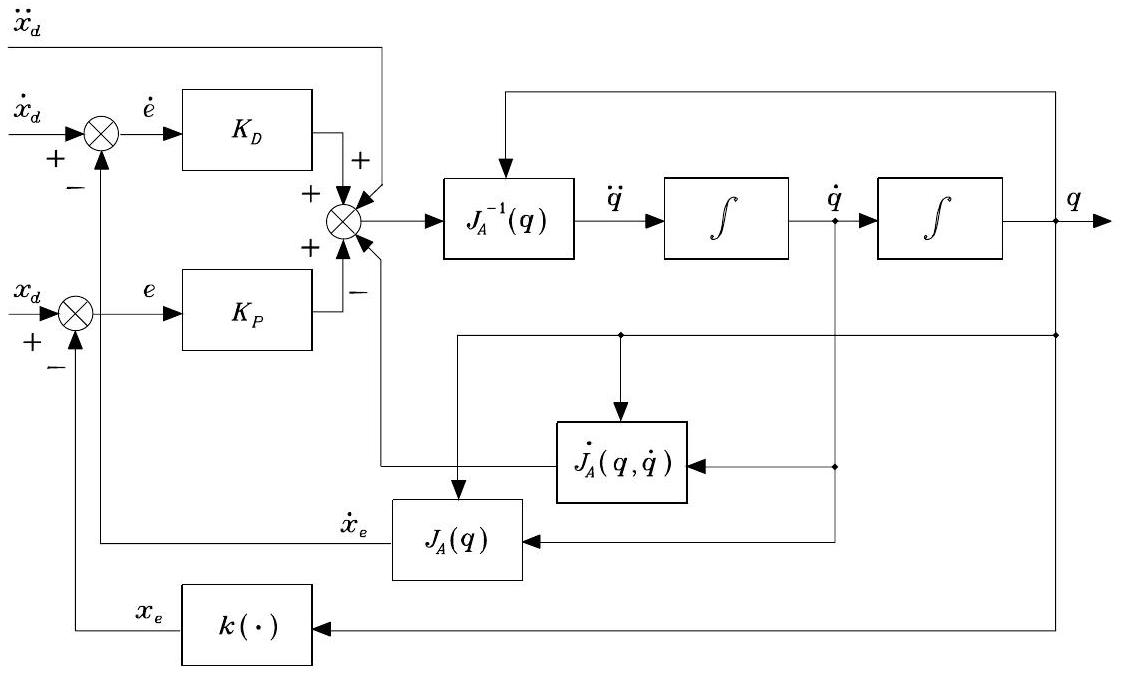
\includegraphics[max width=0.5\textwidth]{diff_kinematics/IK_second_order.jpg}
    \caption{Block scheme of the second-order inverse kinematics algorithm with Jacobian inverse}
    \label{fig:enter-label111}
\end{figure}


In the case of a redundant manipulator, the controller is

$$
\ddot{\boldsymbol{q}}=\boldsymbol{J}_{A}^{\dagger}\left(\ddot{\boldsymbol{x}}_{d}+\boldsymbol{K}_{D} \dot{\boldsymbol{e}}+\boldsymbol{K}_{P} \boldsymbol{e}-\dot{\boldsymbol{J}}_{A}(\boldsymbol{q}, \dot{\boldsymbol{q}}) \dot{\boldsymbol{q}}\right)+\left(\boldsymbol{I}_{n}-\boldsymbol{J}_{A}^{\dagger} \boldsymbol{J}_{A}\right) \ddot{\boldsymbol{q}}_{0}
$$

where the vector $\ddot{\boldsymbol{q}}_{0}$ represents arbitrary joint accelerations chosen to optimize another objective function.







\end{document}